\tikzset{
  estilo nodos/.style={
      node distance=2.5cm,
      estado/.style={circle, draw, minimum size=1cm, inner sep=0pt},
      proba/.style={-latex, thin, bend left=20pt},
      every node/.style={font={\tiny}},
    },
  add flechas/.code={
      \draw[proba] (0) to node[above] {rec.} (1);
      \draw[proba] (1) to node[above] {rec.} (2);
      \draw[proba] (2) to node[above] {$\dots$} (dots.north west);
      \draw[proba] (dots.north east) to node[above] {$\dots$} (n-2);
      \draw[proba] (n-2) to node[above] {rec.} (n-1);
      \draw[proba] (n-1) to node[above] {rec.} (n);
    },
}
\begin{enunciado}{\ejercicio[ÍndiceEspejo]}
  \textit{ÍndiceEspejo}

  Tenemos un arreglo $a = [a_1, \ldots, a_n]$ de $n$ enteros
  distintos (positivos y negativos) \textit{en orden estrictamente creciente}.
  Queremos determinar si existe una posición $i$ tal que $a_i = i$.
  Por ejemplo, dado el arreglo $a = [-4,-1,2,4,7],\, i = 4$ es esa posición.

  Diseñar un algoritmo dividir y conquistar eficiente (cuya complejidad sea de un orden
  estrictamente menor que lineal) que resuelva el problema.
  Calcule y justifique la complejidad del algoritmo dado.
\end{enunciado}

Una complejidad de orden menor a $n$, puede ser algo como $\sqrt{n}$ o muy probablemente algo como $\log(n)$, \textit{because árboles}.

\bigskip

Lo primero que hago es cargar \textit{binarySearch} en el \brain, porque tiene una complejidad $\Theta(\log(n))$ y también funciona
para arreglos ordenados, \textit{moooooy parecido}.

Sobre este algoritmo en particular:
\parrafoDestacado{
  \it
  Me fijo si el índice medio del arreglo es igual al valor $i = A[i]$. Si lo es, gané. Sino tengo que ir para la derecha
  o izquierda según la comparación (¡Arreglo ordenado!).
  Hago así hasta que encuentre un valor verdadero o me quede sin arreglo. Fin.
}

\begin{tcolorbox}
  \begin{lstlisting}[
      mathescape=true,
      emph={[1]funcion, return, ret, retorno},
      emph={[2]si, sino, if, else, true, false},
      emph={[3]indiceEspejo},
      emphstyle={[1]\color{violet}\it},
      emphstyle={[2]\color{red}\it},
      emphstyle={[3]\color{OliveGreen}\it},
      morecomment={[l]{//}},
      commentstyle={\color{gray}\it\footnotesize}
  ]
  funcion indiceEspejo(A[1..n])
    si n = 0  // vacío.
        ret false

    m $\ot$ n/2 // agarra el de abajo, no me importa mucho el caso borde. YOLO.
    si m = A[m]
        ret true
    sino
        si m > A[m]
            ret indiceEspejo(A[m+1..n]) // busco a la der de m.
        sino
            ret indiceEspejo(A[1..m-1]) // busco a la izq de m. \end{lstlisting}
\end{tcolorbox}

% \codigoCpp{ej-4/codigo1-1.cpp}

La función de costo, pa' calcular el \textit{running Time}:
$$
  T(n)=
  \llave{ccl}{
    1 & \text{si} & n = 1 \\
    T(n/2) + 1 & \text{si} & n > 1
  }
$$

Como el costo de resolver cada subproblema es constante, es decir no depende de $n$,
esta función se calcula fácil solo contando los nodos del árbol de recursión.
Árbol que en este caso tiene una sola rama, porque por cada recursión se llama como mucha \ul{una sola} vez
a la función.
Después de todo lo único que hago es una comparación en cada iteración y nada más.
$$
  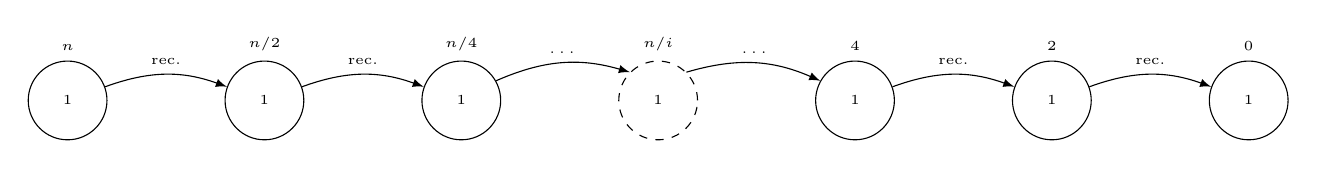
\begin{tikzpicture}[estilo nodos]
    \node[estado, label=above:{$n$}] (0) {$1$};
    \node[estado, right of=0, label=above:{$n/2$}] (1) {$1$};
    \node[estado, right of=1, label=above:{$n/4$}] (2) {$1$};
    \node[estado, right of=2, label={$n/i$}, dashed] (dots) {$1$};
    \node[estado, right of=dots, label=above:{$4$}] (n-2) {$1$};
    \node[estado, right of=n-2, label=above:{$2$}] (n-1) {$1$};
    \node[estado, right of=n-1, label=above:{$0$}] (n) {$1$};

    \draw[proba] (0) to node[above] {rec.} (1);
    \draw[proba] (1) to node[above] {rec.} (2);
    \draw[proba] (2) to node[above] {$\dots$} (dots.north west);
    \draw[proba] (dots.north east) to node[above] {$\dots$} (n-2);
    \draw[proba] (n-2) to node[above] {rec.} (n-1);
    \draw[proba] (n-1) to node[above] {rec.} (n);
  \end{tikzpicture}
$$
¿Cuántos niveles, o para este caso particular, nodos tiene? Tiene $\log_2(n)$. Lo cuál se calcula como la cantidad
$k$ de veces que tengo que dividir el input hasta dar con el caso base.
$$
  T(n/2^k) = T(1) \sii n/2^k = 1 \sii n = 2^k \sii k = \log_2(n)
$$

Por lo tanto la complejidad es:
$$
  \cajaResultado{
    T(n) = \Theta(\log(n))
  }
$$

Con el \textit{Teorema Maestro:}
$$
  T(n) =
  \Theta\big(
  n^{\log_{\blue{b}}(\magenta{a})} \log^{k+1}(n)
  \big)
  \Entonces{$\blue{b} = 2 \ytext \magenta{a} = 1$}[$k = 0$]
  \cajaResultado{
    T(n) =
    \Theta\big(
    \log(n)
    \big)
  }
$$

\fin
